\chapter{System Analysis and Design}
\label{chap:design}
\begin{spacing}{1.2}
\minitoc
\thispagestyle{MyStyle}
\end{spacing}
\newpage

\section{Introduction}

This chapter turns the problem and objectives stated in
Chapter~\ref{chap:context} into a concrete design: it specifies the
functional and non-functional requirements the system must satisfy,
identifies its actors and the use cases they exercise, presents the
dynamic view of the system as a sequence diagram of its end-to-end flow,
presents the static view as a class diagram of its Odoo data model, and
closes with the design philosophy and system architecture that these
requirements led to. Chapter~\ref{chap:implementation} then covers how
this design was actually implemented and evaluated.

% ─────────────────────────────────────────────
\section{Requirements Specification}

\subsection{Functional Requirements}

\renewcommand{\arraystretch}{1.35}
\begin{longtable}{|p{1.3cm}|p{11.8cm}|}
\hline
\textbf{ID} & \textbf{Requirement} \\
\hline
\endhead
\textit{FR1} & Read a named field's value from an uploaded supplier document, using
a deterministic regex pre-parser for known templated fields, with a
fallback to LLM-grounded reading of the raw document text when no pattern
matches. \\
\hline
\textit{FR2} & Look up a versioned default emission factor for a given sector,
production route, and country as of the declaration date, rejecting an
ambiguous match (zero or more than one candidate record) rather than
resolving it silently. \\
\hline
\textit{FR3} & Deterministically compute embedded emissions and certificate
liability for a declaration line from validated inputs, with zero
language-model involvement in the arithmetic itself. \\
\hline
\textit{FR4} & Run an advisory self-consistency check on extracted data before the
final write, including grounding any actual-sourced emissions value
against document text genuinely extracted earlier in the same job. \\
\hline
\textit{FR5} & Escalate a declaration line to human review, either explicitly
(model-initiated) or automatically once the iteration cap is reached
without a completed write. \\
\hline
\textit{FR6} & Persist at most one validated write per declaration line per job,
together with the full tool-call trace as an audit record. \\
\hline
\textit{FR7} & Distinguish, on the declaration line, a genuinely exempt line from
one whose certificate figure is zero only because reference data has not
yet been seeded two states that would otherwise be visually identical to
a user. \\
\hline
\textit{FR8} & Scope declarant users to their own declarations, declaration lines,
and source documents; grant managers unrestricted access across all
declarants. \\
\hline
\caption{Functional requirements.}
\label{tab:functional_requirements}
\end{longtable}
\renewcommand{\arraystretch}{1}

\subsection{Non-Functional Requirements}

\renewcommand{\arraystretch}{1.35}
\begin{longtable}{|p{1.3cm}|p{11.8cm}|}
\hline
\textbf{ID} & \textbf{Requirement} \\
\hline
\endhead
\textit{NFR1} & Compliance arithmetic must never depend on a language model's
output; the agent loop may only decide \textit{when} to trigger a
calculation, never perform it. \\
\hline
\textit{NFR2} & Every agent job is bounded to at most 8--10 tool-calling
iterations, with an automatic escalation fallback if the cap is reached
without a terminal state. \\
\hline
\textit{NFR3} & Numeric values submitted for a declaration write are bounded by
hard plausibility limits (quantity, emission-factor magnitude), enforced
independently of the advisory consistency check. \\
\hline
\textit{NFR4} & A measured (``actual'') emissions figure may only be written if
accompanied by a verbatim quote that is a genuine substring of document
text the system itself has already extracted during that job not merely
a plausible-looking string. \\
\hline
\textit{NFR5} & Regulatory reference data (emission factors, benchmarks, year
parameters) is held in versioned, citation-bearing database tables; no
compliance constant may be hardcoded in application code. \\
\hline
\textit{NFR6} & Uploaded document attachments are size-capped, with the limit
enforced independently at both upload time and read time. \\
\hline
\textit{NFR7} & The orchestrator's job API fails closed: an unconfigured API key
rejects every request rather than disabling authentication, and key
comparison is constant-time. \\
\hline
\textit{NFR8} & The deployment is data-sovereign: the only external network
dependency is the private VPN mesh between the two project-owned
machines; neither host makes a third-party API call. \\
\hline
\caption{Non-functional requirements.}
\label{tab:nonfunctional_requirements}
\end{longtable}
\renewcommand{\arraystretch}{1}

% ─────────────────────────────────────────────
\section{Actors and Use Cases}

The system's own access-control configuration distinguishes exactly two
human-facing actors. The \textbf{Declarant} is row-scoped to their own
declarations, declaration lines, and source documents, while the
\textbf{Manager} has unrestricted access across every declarant --- a
generalisation relationship, since a Manager can do everything a
Declarant can, plus manage shared reference data.

One further point is worth making precise here, since it shapes how the
loop itself should be read as a security diagram: the \textbf{Agent Loop
(LLM)} is modelled as a \textit{secondary, system} actor, not an
independently privileged one. The orchestrator authenticates to Odoo as a
single privileged service account for every job, so the agent loop is
never itself subject to Odoo's row-level security. It is invoked by a
Declarant's own trigger action, and is instead scoped to the correct
declaration and declaration line entirely in application code
(Section~\ref{sec:related_work_cbam} already explained why no LLM-facing
argument is trusted for this scoping).

\begin{figure}[H]
\centering
\begin{tikzpicture}[
  actor/.style={rectangle, rounded corners=4pt, draw=gray!70, fill=gray!8,
                text width=2.5cm, align=center, font=\small, minimum height=0.9cm},
  usecase/.style={ellipse, draw=blue!60, fill=blue!6, text width=3.1cm,
                  align=center, font=\small, minimum height=1.0cm},
  rel/.style={thick},
  incl/.style={thick, dashed, -{Stealth[length=5pt]}},
  gen/.style={thick, -{Triangle[open, length=7pt]}},
]
\node[actor] (declarant) {Declarant};
\node[usecase, right=2.4cm of declarant] (uc1) {Upload Supplier Document};
\node[usecase, below=0.4cm of uc1] (uc2) {Trigger Declaration Processing};
\node[usecase, below=0.4cm of uc2] (uc3) {Run Agentic Extraction Loop};
\node[usecase, below=0.4cm of uc3] (uc4) {Escalate for Human Review};
\node[usecase, below=0.4cm of uc4] (uc5) {Review / Correct Declaration};
\node[usecase, below=0.4cm of uc5] (uc6) {Monitor Job Status};
\node[usecase, below=0.4cm of uc6] (uc7) {Manage Reference Data};

\node[actor, below=1.6cm of uc7, xshift=-6.2cm] (manager) {Manager};
\node[actor, right=2.8cm of uc3] (agent) {Agent Loop (LLM)};

\draw[rel] (declarant) -- (uc1);
\draw[rel] (declarant) -- (uc2);
\draw[rel] (declarant) to[out=290, in=180] (uc5.west);
\draw[rel] (declarant) -- (uc6);
\draw[rel] (manager) -- (uc7);
\draw[gen] (manager) -- (declarant);
\draw[incl] (uc2) -- node[above, font=\scriptsize]{\textit{include}} (uc3);
\draw[incl] (uc4) -- node[above, font=\scriptsize]{\textit{extend}} (uc3);
\draw[rel] (agent) -- (uc3);

\node[draw=gray!50, dashed, rounded corners=6pt,
      fit=(uc1)(uc2)(uc3)(uc4)(uc5)(uc6)(uc7), inner sep=10pt,
      label={[font=\footnotesize\itshape, gray!70]above:CBAM Declaration Automation System}] {};
\end{tikzpicture}
\vspace{0.2cm}
\caption{Use case diagram of the CBAM Declaration Automation System.}
\label{fig:usecase_cbam}
\end{figure}
\FloatBarrier

Table~\ref{tab:usecases_cbam} summarises each use case's actor(s) and
intent.

\begin{table}[H]
\centering
\begin{tabular}{|p{4.0cm}|p{2.4cm}|p{6.6cm}|}
\hline
\textbf{Use Case} & \textbf{Actor(s)} & \textbf{Description} \\
\hline
Upload Supplier Document & Declarant & Attach a document to a declaration line as a \texttt{cbam.source.document} record. \\
\hline
Trigger Declaration Processing & Declarant & Start an orchestrator job for one declaration line; includes \textit{Run Agentic Extraction Loop}. \\
\hline
Run Agentic Extraction Loop & Agent Loop & The ReAct-style loop from Chapter~\ref{chap:context}, executing the seven tools described in Chapter~\ref{chap:implementation} until it writes or escalates. \\
\hline
Escalate for Human Review & Agent Loop & Extends the loop: triggered explicitly by the model, or automatically once the iteration cap is reached. \\
\hline
Review / Correct Declaration & Declarant, Manager & Inspect a line's extracted values, certificate status, and audit trail after a job completes. \\
\hline
Monitor Job Status & Declarant, Manager & Poll a job's status, iteration count, and tool-call/reasoning-turn counters. \\
\hline
Manage Reference Data & Manager & Maintain emission factors, benchmarks, year parameters, goods, installations, and production routes. \\
\hline
\end{tabular}
\caption{Use case descriptions.}
\label{tab:usecases_cbam}
\end{table}
\FloatBarrier

% ─────────────────────────────────────────────
\section{Dynamic View: Sequence Diagram}

Figure~\ref{fig:sequence_cbam} traces \textit{Trigger Declaration
Processing} end to end, across the four participants introduced above:
the Declarant, Odoo (the Softworker host), the Orchestrator (the FastAPI
agent-loop service, also on the Softworker host), and the LLM (served by
Ollama on the Hardworker host). Only the Orchestrator--LLM exchange
crosses the Tailscale VPN between the two machines; every
Orchestrator--Odoo exchange is an RPC call over the Softworker's own
internal Docker network.

\begin{figure}[H]
\centering
\begin{tikzpicture}[
  lifeline/.style={dashed, gray!60, thick},
  head/.style={rectangle, rounded corners=3pt, draw=gray!70, fill=gray!8,
               text width=2.6cm, align=center, font=\small, minimum height=0.8cm},
  msg/.style={-{Stealth[length=5pt]}, thick},
  ret/.style={-{Stealth[length=5pt]}, thick, dashed},
  lbl/.style={font=\scriptsize, align=center},
]
% Lifeline headers
\node[head] (h1) at (0,0)  {Declarant};
\node[head] (h2) at (4.4,0) {Odoo (Softworker)};
\node[head] (h3) at (8.8,0) {Orchestrator};
\node[head] (h4) at (13.2,0) {LLM (Hardworker)};

\draw[lifeline] (h1.south) -- ++(0,-15.1);
\draw[lifeline] (h2.south) -- ++(0,-15.1);
\draw[lifeline] (h3.south) -- ++(0,-15.1);
\draw[lifeline] (h4.south) -- ++(0,-15.1);

% Messages, y decreasing
\draw[msg] (0,-0.9) -- node[lbl, above]{1: upload document} (4.4,-0.9);
\draw[msg] (0,-1.6) -- node[lbl, above]{2: trigger processing} (4.4,-1.6);
\draw[msg] (4.4,-2.3) -- node[lbl, above]{3: POST /jobs \{declaration\_id, line\_id\}} (8.8,-2.3);
\draw[ret] (8.8,-3.0) -- node[lbl, above]{4: 202 Accepted, job\_id} (4.4,-3.0);
\draw[msg] (8.8,-3.7) -- node[lbl, above]{5: RPC read line context} (4.4,-3.7);
\draw[ret] (4.4,-4.4) -- node[lbl, above]{6: good, installation, docs} (8.8,-4.4);

\draw[gray!50, thick] (7.6,-5.0) rectangle (14.0,-9.7);
\node[font=\scriptsize\itshape, gray!60] at (10.8,-5.2) {loop [max 8--10 iterations]};

\draw[msg] (8.8,-5.9) -- node[lbl, above]{7: chat(messages)} (13.2,-5.9);
\draw[ret] (13.2,-6.6) -- node[lbl, above]{8: tool\_calls[]} (8.8,-6.6);
\draw[msg] (8.8,-7.3) -- node[lbl, above]{9: RPC extract\_field /} (4.4,-7.3);
\node[lbl] at (6.6,-7.55) {lookup\_default\_value};
\draw[ret] (4.4,-8.2) -- node[lbl, above]{10: document text / factor} (8.8,-8.2);
\draw[msg] (8.8,-8.9) -- node[lbl, above]{11: tool result(s)} (13.2,-8.9);

\draw[gray!50, thick] (2.2,-10.3) rectangle (14.0,-12.6);
\node[font=\scriptsize\bfseries, gray!60] at (2.55,-10.45) {alt};
\node[lbl, font=\scriptsize\itshape] at (8.5,-10.5) {[write\_declaration\_line called]};
\draw[msg] (8.8,-11.0) -- node[lbl, above]{12: RPC write (single-write guard)} (4.4,-11.0);
\draw[gray!50, dashed] (2.2,-11.35) -- (14.0,-11.35);
\node[lbl, font=\scriptsize\itshape] at (8.5,-11.55) {[escalated / exhausted / no\_write]};
\node[lbl, font=\scriptsize, text=gray!60, text width=9.2cm] at (8.1,-12.1)
  {no RPC --- \texttt{write\_declaration\_line} was never called; the
  declaration line is left untouched};

\draw[msg] (8.8,-13.3) -- node[lbl, above]{13: RPC write\_llm\_trace (audit; always runs, either branch)} (4.4,-13.3);
\draw[msg] (0,-14.0) -- node[lbl, above]{14: GET /jobs/\{id\}/status (poll)} (8.8,-14.0);
\draw[ret] (8.8,-14.7) -- node[lbl, above]{15: status, iterations, counters} (0,-14.7);
\end{tikzpicture}
\vspace{0.2cm}
\caption{Sequence diagram for \textit{Trigger Declaration Processing}.}
\label{fig:sequence_cbam}
\end{figure}
\FloatBarrier

Solid arrows above are calls and dashed arrows are returns. Steps 7--11
repeat inside the bounded loop; step 9 is a stand-in for whichever
read-only tool the model calls (\texttt{calculate\_emissions} and
\texttt{check\_consistency} are pure computation and never leave the
Orchestrator). The diagram deliberately does not show only the happy
path: step 12 runs, at most once per job, only in the branch where the
model actually called \texttt{write\_declaration\_line} before the loop
ended. In every other outcome --- an explicit escalation, the iteration
cap being exhausted, or the loop ending without a write --- no
declaration-line RPC happens at all, and the job produces nothing for a
human to review beyond the audit trace. Step 13, by contrast, is
unconditional: \texttt{write\_llm\_trace} runs on every job regardless of
which branch was taken, recording \texttt{extraction\_status} as
\texttt{extracted} only in the first case and \texttt{needs\_review} in
every other one (\texttt{softworker/orchestrator/main.py}'s
\texttt{\_EXTRACTION\_STATUS\_BY\_LOOP\_STATUS} mapping).

% ─────────────────────────────────────────────
\section{Static View: Data Model}
\label{sec:data_model_cbam}

The domain is modelled as nine Odoo models, all in the custom \texttt{cbam}
addon. Figure~\ref{fig:class_cbam} shows the seven models most central to a
declaration line's own data; \texttt{cbam.good.benchmark} and
\texttt{cbam.year.parameter} are described in the accompanying text rather
than drawn, to keep the figure legible.

\begin{figure}[H]
\centering
\resizebox{\textwidth}{!}{%
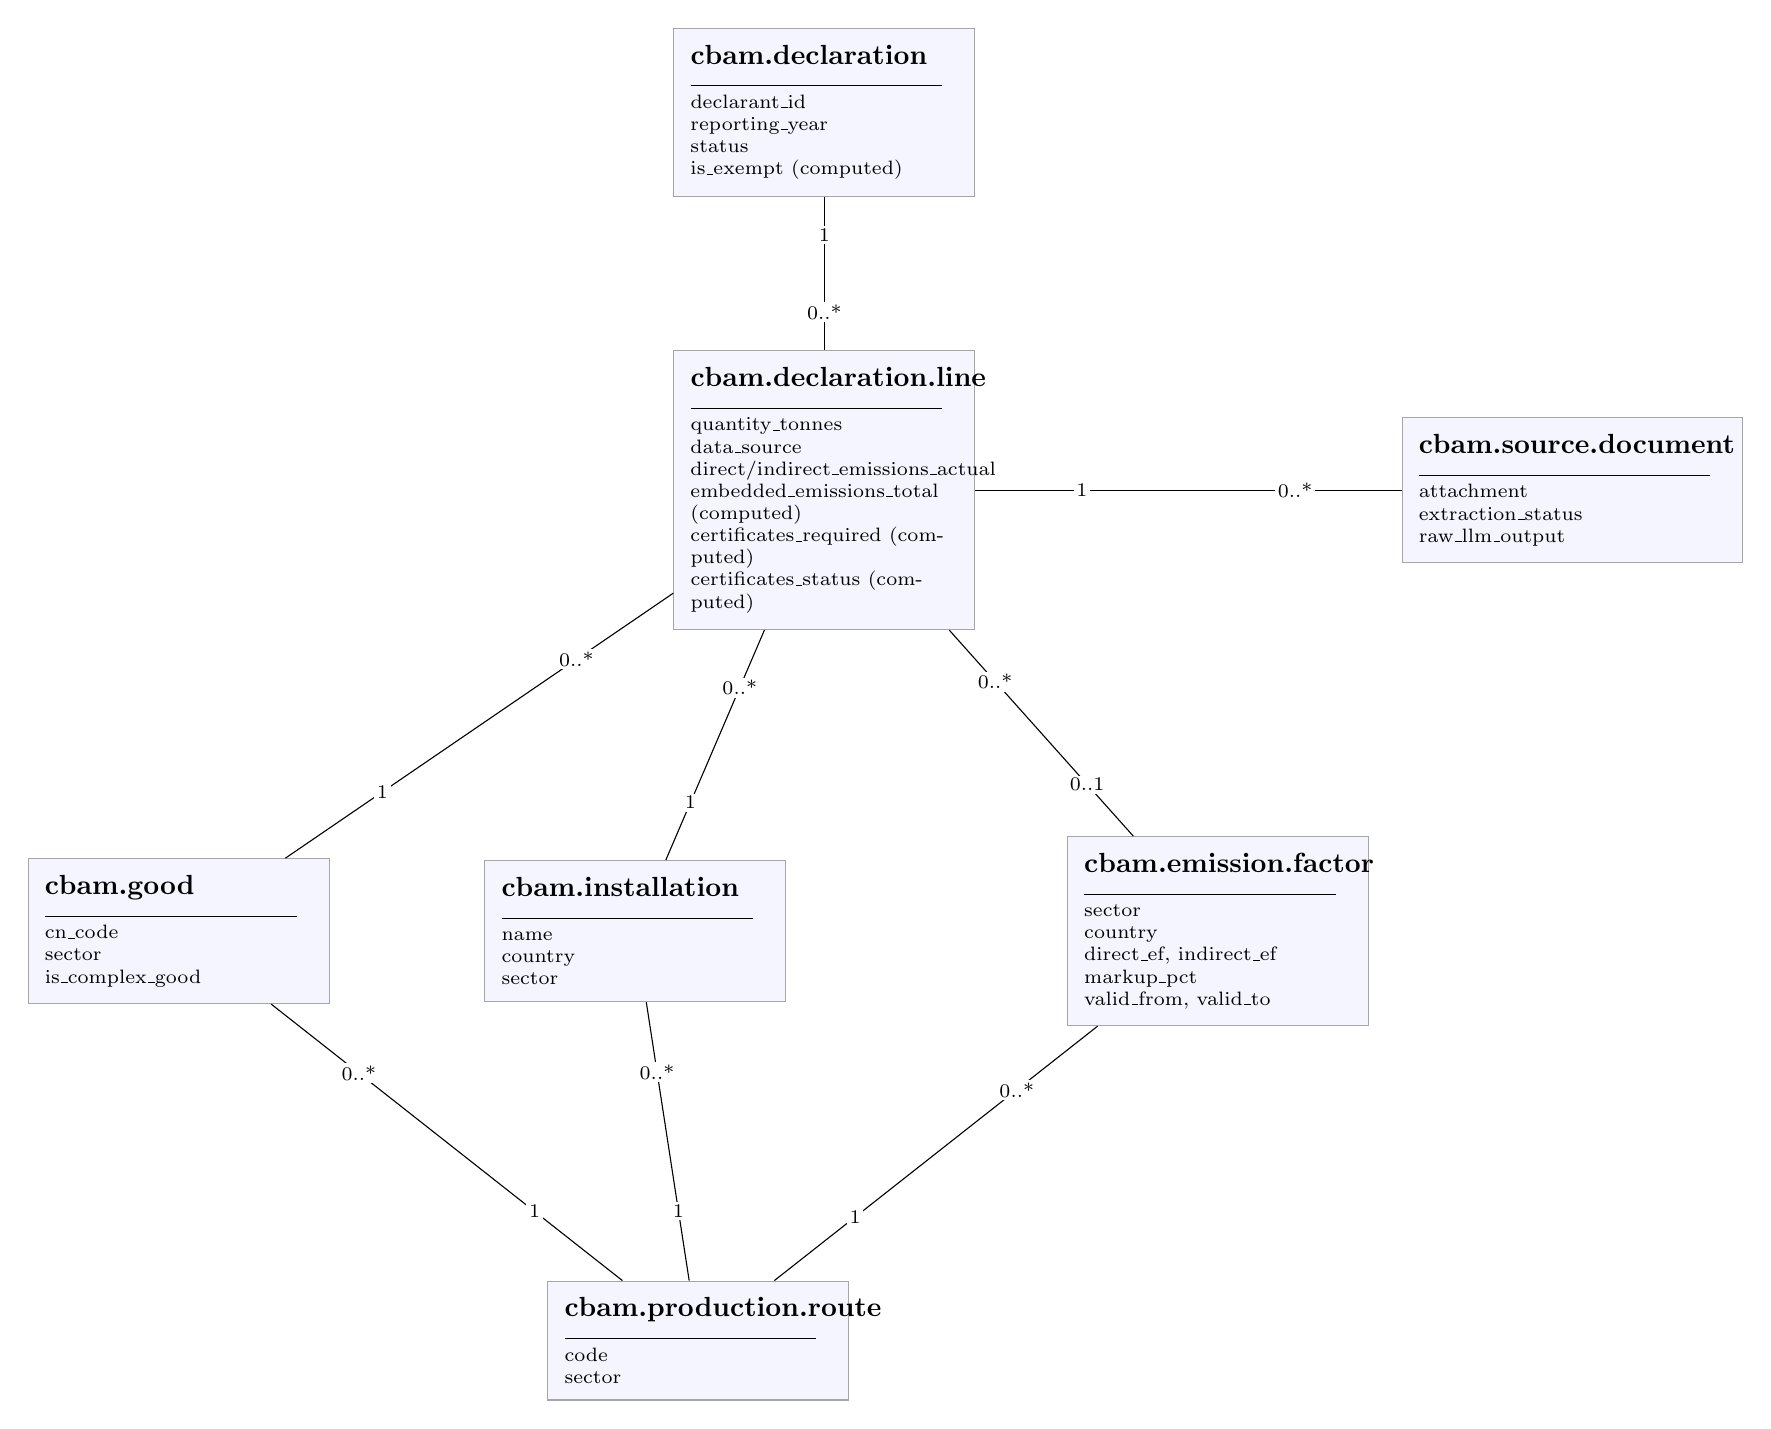
\begin{tikzpicture}[
  class/.style={rectangle, draw=gray!70, fill=blue!4, align=left,
                text width=3.4cm, font=\scriptsize, inner sep=6pt},
  edgelbl/.style={font=\scriptsize, fill=white, inner sep=1pt},
]
\node[class] (decl) at (7,0) {
  \textbf{\normalsize cbam.declaration}\\
  \rule{3.2cm}{0.3pt}\\
  declarant\_id\\ reporting\_year\\ status\\ is\_exempt (computed)
};
\node[class] (line) at (7,-4.8) {
  \textbf{\normalsize cbam.declaration.line}\\
  \rule{3.2cm}{0.3pt}\\
  quantity\_tonnes\\ data\_source\\ direct/indirect\_emissions\_actual\\
  embedded\_emissions\_total (computed)\\ certificates\_required (computed)\\
  certificates\_status (computed)
};
\node[class] (good) at (-1.2,-10.4) {
  \textbf{\normalsize cbam.good}\\
  \rule{3.2cm}{0.3pt}\\
  cn\_code\\ sector\\ is\_complex\_good
};
\node[class] (inst) at (4.6,-10.4) {
  \textbf{\normalsize cbam.installation}\\
  \rule{3.2cm}{0.3pt}\\
  name\\ country\\ sector
};
\node[class] (ef) at (12,-10.4) {
  \textbf{\normalsize cbam.emission.factor}\\
  \rule{3.2cm}{0.3pt}\\
  sector\\ country\\ direct\_ef, indirect\_ef\\ markup\_pct\\
  valid\_from, valid\_to
};
\node[class, text width=3.9cm] (doc) at (16.5,-4.8) {
  \textbf{\normalsize cbam.source.document}\\
  \rule{3.7cm}{0.3pt}\\
  attachment\\ extraction\_status\\ raw\_llm\_output
};
\node[class] (route) at (5.4,-15.6) {
  \textbf{\normalsize cbam.production.route}\\
  \rule{3.2cm}{0.3pt}\\
  code\\ sector
};

\draw (decl) -- node[edgelbl, pos=0.25]{1} node[edgelbl, pos=0.75]{0..*} (line);
\draw (line) -- node[edgelbl, pos=0.25]{0..*} node[edgelbl, pos=0.75]{1} (good);
\draw (line) -- node[edgelbl, pos=0.25]{0..*} node[edgelbl, pos=0.75]{1} (inst);
\draw (line) -- node[edgelbl, pos=0.25]{0..*} node[edgelbl, pos=0.75]{0..1} (ef);
\draw (line) -- node[edgelbl, pos=0.25]{1} node[edgelbl, pos=0.75]{0..*} (doc);
\draw (good) -- node[edgelbl, pos=0.25]{0..*} node[edgelbl, pos=0.75]{1} (route);
\draw (inst) -- node[edgelbl, pos=0.25]{0..*} node[edgelbl, pos=0.75]{1} (route);
\draw (ef) -- node[edgelbl, pos=0.25]{0..*} node[edgelbl, pos=0.75]{1} (route);
\end{tikzpicture}%
}
\vspace{0.2cm}
\caption{Class diagram of the seven core \texttt{cbam} models.}
\label{fig:class_cbam}
\end{figure}
\FloatBarrier

Beyond the associations shown, two reference tables complete the model:
\texttt{cbam.good.benchmark} (a per-good, per-route free-allocation
benchmark, unique per \texttt{good\_id}/\texttt{production\_route\_id}
pair, itself referencing \texttt{cbam.production.route}) and
\texttt{cbam.year.parameter} (the yearly phase-out factor and reference
certificate price, unique per \texttt{year}); \texttt{cbam.declaration.line}
holds a computed reference to each. Several constraints keep this model
internally consistent rather than merely populated: a Python constraint on
\texttt{cbam.declaration.line} rejects a good/installation/route
combination whose sectors disagree; a Python constraint on
\texttt{cbam.emission.factor} rejects a validity range that overlaps an
existing one for the same sector/route/country, so a lookup can never
silently match more than one record; SQL unique constraints enforce one
\texttt{(cn\_code, sector)} per good, one \texttt{(code, sector)} per
production route, and one row per year in \texttt{cbam.year.parameter};
and a size constraint on \texttt{cbam.source.document.attachment} caps
every uploaded document, enforced again independently at read time when
the orchestrator fetches it.

% ─────────────────────────────────────────────
\section{Design Philosophy}
\label{sec:design_philosophy_cbam}

Three principles governed every architectural decision in this project.

\paragraph{Determinism over convenience:} It would be simpler to let the
language model read a document and directly state a certificate liability.
This was ruled out categorically: the compliance number is computed by a
standalone, Odoo-independent Python module, unit-tested against
hand-calculated examples before any LLM code existed, and the agent never
has write access to that computation --- it only decides \textit{when} to
call it.

\paragraph{Autonomy over prescription:} The extraction layer makes its own
decisions about which tool to call, in what order, and how many times,
without a human- or code-authored step sequence. This ruled out a fixed
extraction pipeline in favour of a loop that reasons about the current
conversation state and selects the next action itself, every turn.

\paragraph{Verifiability over assumed capability:} No model was chosen
because of published benchmark scores or model-card claims. Every
candidate was run against the project's own production validation logic,
and --- as Section~\ref{sec:results_cbam} shows --- an initial ranking
obtained this way was itself later found to be a measurement-methodology
artifact and corrected, rather than left unexamined once a plausible
answer had been found.

% ─────────────────────────────────────────────
\section{System Architecture}
\label{sec:architecture_cbam}

The system is deployed across two roles, meshed over a private VPN, as
shown in Figure~\ref{fig:architecture_cbam}.

\begin{figure}[H]
\centering
\begin{tikzpicture}[
  node distance=0.6cm and 1.4cm,
  host/.style={rectangle, rounded corners=6pt, draw=gray!70, thick,
               text width=6.4cm, align=center, minimum height=3.6cm, inner sep=8pt},
  svc/.style={rectangle, rounded corners=3pt, draw=blue!60, fill=blue!7,
              text width=5.6cm, align=center, font=\small, minimum height=0.7cm},
  gate/.style={rectangle, rounded corners=3pt, draw=orange!70, fill=orange!8,
               text width=5.6cm, align=center, font=\small, minimum height=0.7cm},
  arrow/.style={-{Stealth[length=6pt]}, thick},
]
\node[host, label={[font=\bfseries]above:Hardworker (LLM host, GPU-capable)}] (hw) {};
\node[svc, below=0.5cm of hw.north] (ollama) {Ollama\\(local LLM inference)};
\node[gate, below=0.3cm of ollama] (nginx) {nginx\\API-key gate, rate limiting};

\node[host, right=1.9cm of hw, label={[font=\bfseries]above:Softworker (Odoo host)}] (sw) {};
\node[svc, below=0.5cm of sw.north] (pg) {PostgreSQL 16 (internal network only)};
\node[svc, below=0.3cm of pg] (odoo) {Odoo 17 + \texttt{cbam} addon};
\node[svc, below=0.3cm of odoo] (orch) {Orchestrator (FastAPI agent loop)};

\draw[arrow, <->] (nginx.east) -- node[above, font=\scriptsize, text width=1.7cm, align=center]
  {Tailscale VPN (WireGuard, encrypted mesh)} (orch.west |- nginx.east);
\end{tikzpicture}
\vspace{0.3cm}
\caption{System architecture: Hardworker (LLM host) and Softworker (Odoo
host), meshed over a private VPN.}
\label{fig:architecture_cbam}
\end{figure}
\FloatBarrier

Only the Orchestrator--Ollama exchange crosses the VPN shown above. The
originally specified per-role Tailscale sidecar identity had to be
replaced, on \textbf{both} hosts, by each host's own already-authenticated
VPN connection, after a reproducible key-generation fault turned up in
the VPN provider's own console. The fix was applied first to the
Softworker host during live deployment, then pre-emptively mirrored onto
the Hardworker host once the same root cause was recognised --- a
documented deviation, not one silently absorbed into the design.

A user uploads a supplier document in the Odoo UI and triggers processing;
Odoo calls the orchestrator's job endpoint and polls its status while the
agent loop runs against the LLM host over the VPN; on completion the
orchestrator performs a single validated write back to Odoo, and the full
tool-call trace is persisted as an audit trail (Figure~\ref{fig:sequence_cbam}
above gives the precise sequence).

The stack uses Odoo~17 Community, PostgreSQL~16, Ollama for local
inference, FastAPI for the orchestrator, Pydantic for argument validation,
and the plain \texttt{openai} client SDK pointed at Ollama's
OpenAI-compatible endpoint. Deliberately absent is \textbf{any agent
framework} (LangChain, AutoGen, CrewAI): for a fixed, seven-tool schema, a
framework would only add indirection without benefit, and would make the
deterministic-calculation boundary harder to audit.

% ─────────────────────────────────────────────
\section{Conclusion}

This chapter has turned Chapter~\ref{chap:context}'s problem statement
into a concrete design: eight functional and eight non-functional
requirements, two human actors plus the agent loop modelled correctly as
a secondary system actor, a traced end-to-end sequence, and a nine-model
data model built around three deliberate design principles and a
two-machine architecture. Chapter~\ref{chap:implementation} now covers
how this design was implemented --- the calculation engine, the agentic
pipeline built on top of it, and the empirical evaluation of both.
